

\documentclass[11pt,a4paper, french]{article}
\usepackage{hyperref}
\hypersetup{
    colorlinks=true,
    linkcolor=blue,
    filecolor=blue,      
    urlcolor=blue, 
    citecolor=blue
    }

\urlstyle{same}
\usepackage[numbers,sort&compress]{natbib} 

\usepackage[T1]{fontenc} 
\usepackage[french]{babel} 
\usepackage[utf8x]{inputenc}
\usepackage{amsmath}
\usepackage{pdfpages}
\usepackage{amsfonts}
\usepackage{amssymb}
\usepackage[margin=1.5cm, top=1cm, bottom=1.5cm]{geometry}
\usepackage{multicol}
\usepackage{graphicx}
\usepackage{calc}
\usepackage{diagbox}
\usepackage{bbold}
\usepackage{array}
\usepackage{minted}
\usepackage{alltt}
\usepackage{pstricks-add}
\usepackage{pstricks}
\usepackage{amsthm}
% \usepackage{moreverb}
\usepackage{forest}
\usepackage{tikz}
\usepackage{enumerate}


\usepackage[ruled,lined]{algorithm2e}

\usepackage{float}
\usepackage[caption = false]{subfig}

% %\renewcommand{\cite}[1]{\textsuperscript{\citep{#1}}}
% \usepackage{url}
% % Packages pour la mise en page et la personnalisation de la table des matières
% \usepackage{tocloft}    % Permet de personnaliser la table des matières
% \usepackage{titlesec}   % Permet de personnaliser les titres des sections
% \usepackage{lmodern}    % Améliore la police de base
% \usepackage{setspace}   % Pour gérer les espaces dans le document
% 
% % Personnalisation de la table des matières
% \renewcommand{\cftsecfont}{\large\bfseries}  % Sections en gras et en plus grand
% \renewcommand{\cftsecpagefont}{\large\bfseries}  % Numéros de page en gras
% \renewcommand{\cftsubsecfont}{\normalsize\itshape}  % Sous-sections en italique
% \renewcommand{\cftsubsubsecfont}{\normalsize\itshape}  % Soussous-sections en italique
% \renewcommand{\cftsubsecpagefont}{\normalsize\itshape}  % Numéros de sous-sections en italique
% \renewcommand{\cftsubsubsecpagefont}{\normalsize\itshape}  % Numéros de soussous-sections en italique
% \renewcommand{\contentsname}{} % Enlever le "Contents"

\usetikzlibrary{automata}
\usetikzlibrary{calc,arrows.meta,positioning}

\title{\textsc{ADAM: A method for Stochastic Optimization}\\
Résumé d'article}
\author{Guillaume BERNARD-REYMOND, Guillaume BOULAND,\\ Camille MOTTIER, Abel SILLY}
\date{7 octobre 2024}
% \newcommand{\iddots}{\reflectbox{$\ddots$}}


\usetikzlibrary{arrows.meta}

\newcommand{\R}{\mathbb{R}}
\newcommand{\m}{\mathcal}
\newcommand{\un}{\mathbb{1}_n}
\newcommand{\N}{\mathbb{N}}

\newcommand{\vs}[1]{\vspace{#1cm}}
\newcommand{\hs}[1]{\hspace{#1cm}}
\newcommand{\dsum}[2]{\displaystyle\sum_{#1}^{#2}}
\newcommand{\dint}[2]{\displaystyle\int_{#1}^{#2}}
\newcommand{\ben}{\begin{enumerate}}
\newcommand{\een}{\end{enumerate}}
\newcommand{\bit}{\begin{itemize}}
\newcommand{\eit}{\end{itemize}}

\newcommand{\var}{\mathbb{V}\text{ar}}
\newcommand{\cov}{\mathbb{C}\text{ov}}

\setlength{\parindent}{0pt}
\frenchbsetup{StandardLists=true}

\theoremstyle{definition}

\newtheorem{Qu}{Question}


\begin{document}



\maketitle

\


\vspace{1cm}  % Espace entre le titre et la table des matières
\tableofcontents
\vspace{1cm} 

\


\section{Introduction}

L'article \og Adam: A method for Stochastic Optimization \cite{kingma2017adammethodstochasticoptimization}\fg{} a été publié en 2014 (et corrigé jusqu'en 2017) par Diederik P. Kingma (Université d'Amsterdam, OpenAI) et Jimmy Lei Ba (Université de Toronto) dans le cadre de l'\textit{International Conference on Learning Representations} (ICLR) de 2015. 

\

Cet article présente l'algorithme Adam, algorithme d'optimisation stochastique, basé sur une descente de gradient, dans le cadre d'un espace de paramètres à grande dimension.
Outre le fait que cet algorithme est simple à implémenter et nécessite peu de mémoire, il semble offrir une méthode qui marche bien dans un large panel de cas, y compris dans les cas problématiques de gradients parcimonieux ou de fonctions-objectifs non stationnaires. En cela, il combine les qualités d'algorithmes existants au préalable, tels que AdaGrad et RMSProp.

\

L'article présente une description précise de l'algorithme Adam, fournit un résultat de convergence de la méthode et aborde l'apport de l'algorithme Adam vis-à-vis d'autres algorithmes. 



\section{Algorithme Adam}
\subsection{Objectif}
On considère une fonction-objectif stochastique $f(\theta)$ de paramètres $\theta$, qu'on suppose différentiable. L'algorithme Adam est une méthode d'ordre 1 (c'est-à-dire qui repose sur des évaluations de la fonctionnelle $f$ et du gradient $\nabla_{\theta}f$), qui a pour objectif d'optimiser les paramètres $\theta$ afin de minimiser l'espérance $\mathbb E[f(\theta)]$. \\
L'aspect stochastique peut venir d'une fonction-objectif intrinsèquement bruitée ou bien d'un échantillonnage réalisé à chaque pas de l'algorithme. Typiquement, $f$ peut être une fonction perte de la forme \\$f(\theta)=\dsum{i=1}nL(x_i|\theta)$, où le calcul de gradient $\nabla_{\theta}f(\theta)=\dsum{i=1}n\nabla_{\theta}L(x_i|\theta)$ est trop coûteux en nombre d'évaluations de gradients. Il est alors remplacé à chaque itération $t$ de l'algorithme par le calcul de $\nabla_{\theta}f_t(\theta)=\dsum{i\in I_t}{}\nabla_{\theta}L(x_i|\theta)$ pour $I_t$ un sous-échantillon (\textit{mini-batch}) et $f_t$ définie par $f_t(\theta)=\dsum{i\in I_t}{}L(x_i|\theta)$.

\subsection{Description de l'algorithme Adam}

Outre la fonction $f(\theta)$, l'algorithme nécessite la donnée d'un pas $\alpha$, de taux $\beta_1,\beta_2\in[0,1[$, d'une constante de stabilisation numérique $\varepsilon>0$ et de paramètres initiaux $\theta_0$ (valeurs par défaut : $\alpha=0.001$, $\beta_1=0.9$, $\beta_2=0.999$, $\varepsilon=10^{-8}$). Il exécute alors le schéma suivant :


\begin{algorithm}
  \caption{Adam}
  \Entree{$f(\theta)$, $\alpha$, $\beta_1$, $\beta_2$, $\varepsilon$, $\theta_0$}
  $m_0\longleftarrow 0$ \\
  $v_0\longleftarrow 0$ \\  
  $t\longleftarrow 0$ \\
  \Tq{$\theta_t$ ne converge pas}{
    $t\longleftarrow t+1$\\
    $g_t \longleftarrow \nabla_{\theta}f_t(\theta_{t-1})$\\
    $m_t \longleftarrow \beta_1\cdotp m_{t-1}+(1-\beta_1)\cdotp g_t$\\
    $v_t \longleftarrow \beta_2\cdotp v_{t-1}+(1-\beta_2)\cdotp g_t^2$\\
    $\widehat m_t \longleftarrow m_t/(1-\beta_1^t)$\\
    $\widehat v_t \longleftarrow v_t/(1-\beta_2^t)$\\
    $\theta_t \longleftarrow \theta_{t-1}-\alpha\cdotp \widehat m_t/(\sqrt{\widehat v_t}+\varepsilon)$
  }
  \Sortie{$\theta_t$}
\end{algorithm}

Pour comprendre cet algorithme et identifier les apports de la méthode Adam, observons les différentes étapes et comparons-les avec celles d'autres algorithmes classiques de descente de gradient stochastique (présentés dans l'annexe).

\bit
\item $m_t \longleftarrow \beta_1\cdotp m_{t-1}+(1-\beta_1)\cdotp g_t$\\
Fournit une estimation de $\mathbb E[g_t]$ par moyenne mobile à décroissance exponentielle : $m_t=(1-\beta_1)\dsum{i=1}t\beta_1^{t-i}\cdotp g_i$.\\
Permet de garder mémoire des directions de descente précédentes afin d'atténuer les variations liées au bruit de la fonction.\\
On trouve une idée similaire dans l'algorithme SGD  avec moment (algorithme \ref{SGD}).

\item $v_t \longleftarrow \beta_2\cdotp v_{t-1}+(1-\beta_2)\cdotp g_t^2$\\
Fournit une estimation de $\mathbb E[g_t^2]$, là aussi par moyenne mobile à décroissance exponentielle.\\
Permettra, lors de la mise à jour des paramètres, une mise à l'échelle du gradient, c'est-à-dire qu'on ne va pas utiliser le même pas pour tous les paramètres. On ralentit le pas en cas de forte variation liée à un paramètre, et on l'accélère en cas de faible variation. 
On trouve une idée similaire dans les algorithmes AdaGrad (mais sans moyenne mobile, algorithme \ref{adagrad}) et RMSProp (algorithme \ref{rmsprop}). 

\item  $\widehat m_t \longleftarrow m_t/(1-\beta_1^t)$ et 
$\widehat v_t \longleftarrow v_t/(1-\beta_2^t)$\\
Permet de réduire le biais vers 0 de $m_t$ et $v_t$ venant de l'initialisation de $m_0$ et $v_0$ à 0. \\
C'est l'innovation fournie par l'algorithme Adam.
\eit

On peut donc observer que l'algorithme Adam combine les idées fournies par les précédents algorithmes de descente de gradient, telles que la personnalisation des pas à chaque paramètre et la mémorisation du passé par le biais des moyennes mobiles, tout en apportant un élément supplémentaire : la correction des biais des estimateurs des moments d'ordre 1 et 2. 



\section{Points forts de la méthode}

\subsection{Contraction du biais}

La grande différence de l'algorithme Adam par rapport aux autres algorithmes de descente de gradients est fournie par les étapes déterminant $\widehat m_t$ et $\widehat v_t$, qui ont pour effet de contracter le biais des estimateurs des moments $m_t$ de $\mathbb E[g_t]$ et $v_t$ de $\mathbb E[g_t^2]$. En effet, nous avons :
$$\mathbb E[m_t]=(1-\beta_1)\dsum{i=1}t\beta_1^{t-i}\mathbb E[g_i]= \mathbb E[g_t]\underset{<1}{\underbrace{(1-\beta_1^t)}}+\underset{\zeta}{\underbrace{(1-\beta_1)\dsum{i=1}t\beta_1^{t-i}(\mathbb E[g_i]-\mathbb E[g_t])}}$$
avec $\zeta$ qui pourra être rendu petit par un bon choix de $\beta_1$. La division par $(1-\beta_1^t)$ permet donc de réduire le biais de $m_t$. Il en est de même pour $v_t$. \\
En particulier, en cas de gradients parcimonieux (\textit{sparse gradient}) qui nécessitent une bonne mémoire du passé, donc des taux $\beta_1$ et $\beta_2$ grands, le biais obtenu peut être conséquent. Le calcul de $\widehat m_t$ et $\widehat v_t$ peut alors s'avérer pertinent.\\
On pourra se reporter à la figure \ref{biais} de l'annexe, issue de l'article \cite{kingma2017adammethodstochasticoptimization}, pour observer graphiquement l'effet de la correction des biais.


\subsection{Majoration du pas}

Dans l'algorithme Adam, le pas à chaque étape est donné par : $\Delta_t=\alpha\cdotp \widehat m_t/\sqrt{\widehat v_t+\varepsilon}$, où $\varepsilon>0$ évite les divisions par des nombres trop petits. En supposant $\varepsilon=0$, l'article donne la borne suivante du pas : 
$$|\Delta_t|\leqslant \left\{\begin{array}{ll}
\alpha\cdotp (1-\beta_1)/\sqrt{1-\beta_2} & \text{ si }(1-\beta_1)>\sqrt{1-\beta_2}\\
\alpha & \text{ sinon}
\end{array}\right.
$$

La première majoration apparaît en fait dans le cadre de gradients parcimonieux. Dans les autres cas, on a une borne de l'ordre de $\alpha$ : $|\Delta_t|\lessapprox \alpha$.\\
Le choix de $\alpha$ permet donc d'avoir un contrôle sur la taille des pas effectués, et donc de définir une \og zone de confiance\fg{} autour des paramètres $\theta_{t-1}$ dans laquelle on peut se déplacer à partir du calcul du gradient $g_t$.

\subsection{Convergence}

Nous considérons ici le regret de la méthode défini par : 
$$R(T)=\dsum{t=1}Tf_t(\theta_t)-\min_{\theta\in\mathcal X}\dsum{t=1}Tf_t(\theta)$$
pour $f_t$ des fonctions de pertes convexes arbitraires. Le regret fournit une sorte de mesure de performance de la trajectoire suivie par l'algorithme dans la recherche de l'optimum. Cette quantité croît avec le temps $T$, mais l'article fournit, sous certaines hypothèses de majoration des gradients et de l'écart entre les valeurs de $\theta_t$,  la relation suivante, qui garantit une croissance de $R(T)$ contrôlée :
$$\dfrac{R(T)}{T}=O\left(\dfrac 1{\sqrt T}\right)$$

On pourra se référer au résultat récent fourni par l'article de S. Dereich et A. Jentzen \cite{dereich2024convergenceratesadamoptimizer} pour un résultat de convergence presque sure et en norme $L^p$ de $\theta_t$. 

\section{Comparaisons expérimentales}
L'article fournit un certain nombre de graphiques illustrant les performances de différentes méthodes de descentes de gradients utilisées sur les bases de données classiques MNIST et IMDB (présentés en annexe dans la figure \ref{fig:IMDB}). Ceux-ci mettent en évidence la bonne performance de l'algorithme Adam, y compris dans le cas de gradients parcimonieux. \\
Dans la même idée, nous avons comparé ces algorithmes dans le cadre de la base de données fashionMNIST. L'évolution de la fonction-perte en fonction du nombre d'itérations des algorithmes est présentée dans la figure \ref{fig1}. On observe que sur cet exemple, l'algorithme Adam fait aussi bien que les algorithmes RMSProp et Adagrad, et nettement mieux que SGD avec moment. 



\begin{figure}[H]
\centering
 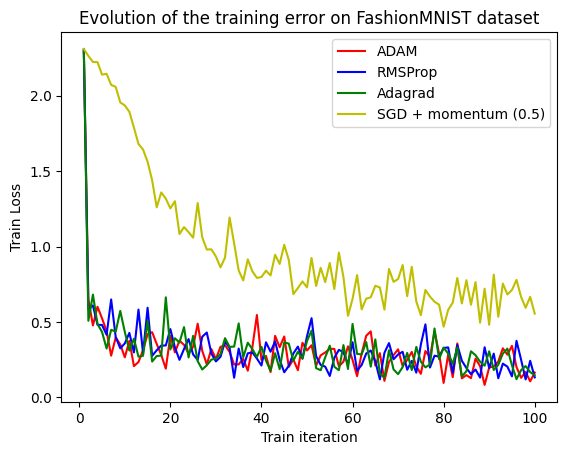
\includegraphics[width=8cm]{Images/FashionMNIST.png}
\caption{Évolution de l'erreur d'entraînement pour la base de données \textit{FashionMNIST}, 10 epochs avec des batchs de taille 64, avec la fonction de perte \textit{Cross Entropy} (code sur \cite{github})}
\label{fig1}
\end{figure}

\vs2

\nocite{kingma2017adammethodstochasticoptimization}
\nocite{starmer2023optimization}
\nocite{dereich2024convergenceratesadamoptimizer}
\nocite{github}
\renewcommand{\refname}{Sources}
\bibliographystyle{unsrt}  % Style de bibliographie
\bibliography{sources}  % Nom du fichier .bib sans l'extension

\newpage

\section{Annexes}

\subsection{Algorithmes de descente de gradients}
\begin{algorithm*}
  \caption{SGD}
  \Entree{$f(\theta)$, $\alpha$, $\theta_0$}
  $t\longleftarrow 0$ \\
  \Tq{$\theta_t$ ne converge pas}{
    $t\longleftarrow t+1$\\
    $g_t \longleftarrow \nabla_{\theta}f_t(\theta_{t-1})$\\
    $\theta_t \longleftarrow \theta_{t-1}-\alpha \cdotp g_t(\theta_{t-1})$
  }
  \Sortie{$\theta_t$}
\end{algorithm*}



\begin{algorithm*}
  \caption{SGD avec moment (1964)}
  \Entree{$f(\theta)$, $\alpha$, $\rho$, $\theta_0$} 
  $t\longleftarrow 0$ \\
  \Tq{$\theta_t$ ne converge pas}{
    $t\longleftarrow t+1$\\
    $g_t \longleftarrow \nabla_{\theta}f_t(\theta_{t-1})$\\
    $m_t \longleftarrow \rho \cdotp m_{t-1}-\alpha \cdotp g_t$\\
    $\theta_t \longleftarrow \theta_{t-1}+m_t$
  }
  \Sortie{$\theta_t$}
  \label{SGD}
\end{algorithm*}



\begin{algorithm*}
  \caption{AdaGrad (2011)}
  \Entree{$f(\theta)$, $\alpha$, $\varepsilon$, $\theta_0$}
  $v_0\longleftarrow 0$ \\  
  $t\longleftarrow 0$ \\
  \Tq{$\theta_t$ ne converge pas}{
    $t\longleftarrow t+1$\\
    $g_t \longleftarrow \nabla_{\theta}f_t(\theta_{t-1})$\\
    $v_t \longleftarrow  v_{t-1}+ g_t^2$\\
    $\theta_t \longleftarrow \theta_{t-1}-\alpha\cdotp g_t/(\sqrt{ v_t}+\varepsilon)$
  }
  \Sortie{$\theta_t$}
  \label{adagrad}
\end{algorithm*}


\begin{algorithm*}[h!]
  \caption{RMSProp (2012)}
  \Entree{$f(\theta)$, $\alpha$, $\beta_2$, $\varepsilon$, $\theta_0$}
  $v_0\longleftarrow 0$ \\  
  $t\longleftarrow 0$ \\
  \Tq{$\theta_t$ ne converge pas}{
    $t\longleftarrow t+1$\\
    $g_t \longleftarrow \nabla_{\theta}f_t(\theta_{t-1})$\\
    $v_t \longleftarrow \beta_2\cdotp v_{t-1}+(1-\beta_2)\cdotp g_t^2$\\
    $\theta_t \longleftarrow \theta_{t-1}-\alpha\cdotp g_t/(\sqrt{v_t}+\varepsilon)$
  }
  \Sortie{$\theta_t$}
  \label{rmsprop}
\end{algorithm*}

\subsection{Illustrations graphiques}
\begin{figure}[H]
    \centering
    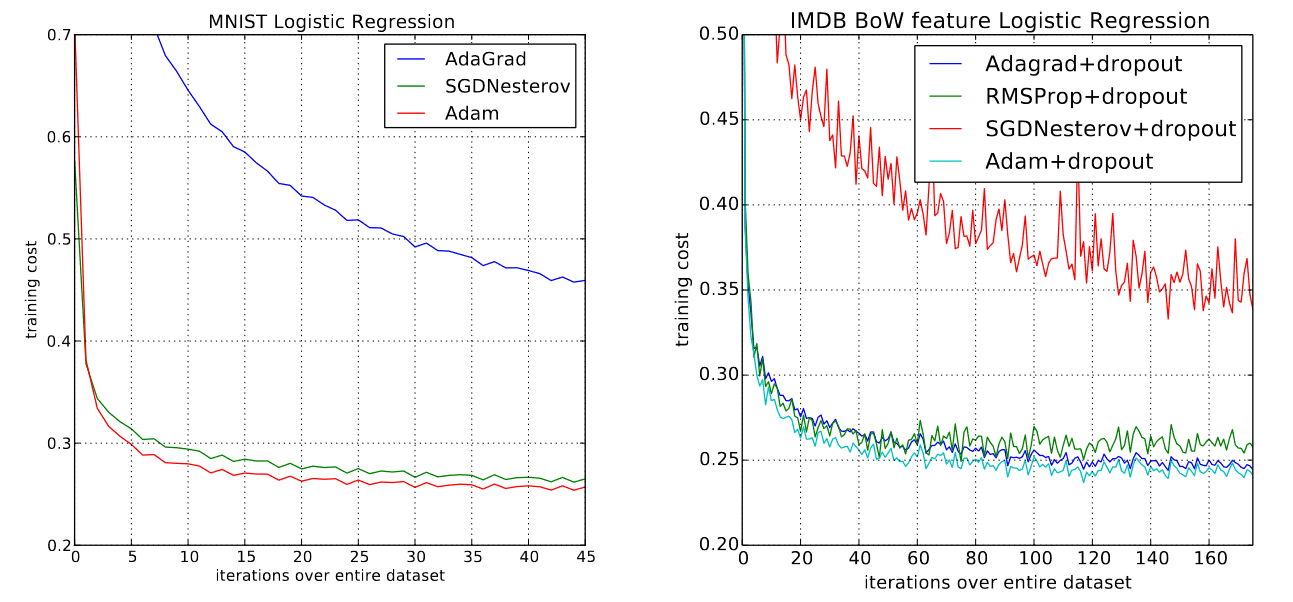
\includegraphics[width=14cm]{Images/IMDB_MNIST_article.png}
    \caption{Régression logistique entraînée sur la fonction de perte de vraisemblance logarithmique négative sur les bases de données d'images MNIST et de critique de films IMDB avec 10000 vecteurs caractéristiques de sacs de mots (\textit{bag-of-words}) (issues de l'article \cite{kingma2017adammethodstochasticoptimization}).}
    \label{fig:IMDB}
\end{figure}

\begin{figure}[H]
    \centering
    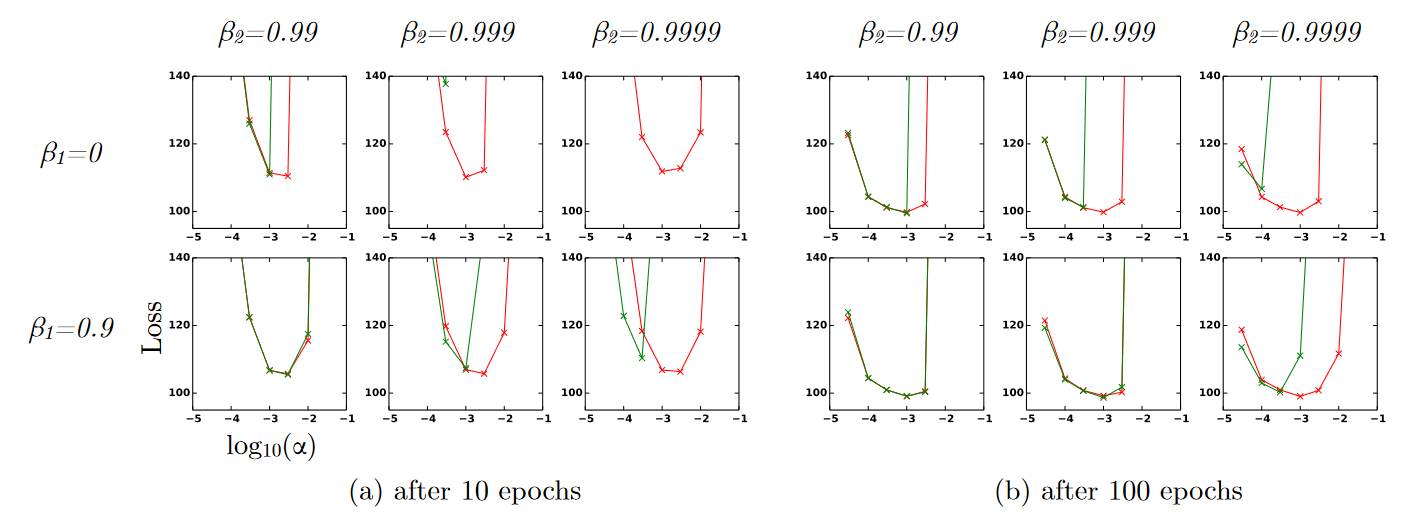
\includegraphics[width=\linewidth]{Images/bias_correction_article.png}
    \caption{Effet de la correction de biais (en rouge, avec correction, en vert, sans correction) après 10 epochs et 100 epochs sur la perte (ordonnées) lors de l'apprentissage d'un VAE pour différents paramétrages de $\alpha$, $\beta_1$, $\beta_2$}
    \label{biais}
\end{figure}
\end{document}


